\documentclass[11pt, a4paper]{article}

% --- Typography and Language ---
\usepackage[utf8]{inputenc}
\usepackage[T1]{fontenc}
\usepackage{lmodern}            % Better standard font
\usepackage{microtype}          % Greatly improves text justification
\usepackage[english]{babel}
\usepackage{csquotes}

% --- Layout and Formatting ---
\usepackage{geometry}
\geometry{margin=1in}
\usepackage{parskip}            % Adds space between paragraphs, removes indentation
\usepackage{titlesec}
\usepackage{fancyhdr}           % Professional headers/footers
\usepackage{lastpage}           % Reference total page count

% --- Graphics and Diagrams ---
\usepackage{graphicx}
\usepackage{tikz}
\usetikzlibrary{positioning, shapes.geometric, arrows.meta, shadows, calc}

% --- Tables and Lists ---
\usepackage{booktabs}           % Professional tables
\usepackage{longtable}
\usepackage{enumitem}

% --- Code Highlighting ---
\usepackage{listings}
\usepackage{xcolor}

% --- Colors ---
\definecolor{primaryblue}{RGB}{0, 51, 102}
\definecolor{accentblue}{RGB}{0, 102, 204}
\definecolor{codegreen}{rgb}{0,0.6,0}
\definecolor{codegray}{rgb}{0.5,0.5,0.5}
\definecolor{codepurple}{rgb}{0.58,0,0.82}
\definecolor{backcolour}{rgb}{0.97,0.97,0.97}

% --- Hyperlinks (Must be last) ---
\usepackage{hyperref}
\hypersetup{
    colorlinks=true,
    linkcolor=primaryblue,
    filecolor=magenta,      
    urlcolor=accentblue,
    pdftitle={Pectra Phase 2: EOFv1 Integration Report},
    pdfauthor={Germina Labs}
}

% --- Listing Style ---
\lstdefinelanguage{Rust}{
  keywords={fn, let, mut, if, else, loop, match, return, pub, struct, enum, impl, use, mod, crate, const, true, false, for, while, type},
  keywordstyle=\color{magenta},
  ndkeywords={self, Self, u8, u16, u32, u64, usize, i8, i16, i32, i64, isize, f32, f64, bool, char, str, String, Vec, Option, Result, Box},
  ndkeywordstyle=\color{codepurple},
  morecomment=[l]{//},
  morecomment=[s]{/*}{*/},
  commentstyle=\color{codegreen},
  stringstyle=\color{codepurple},
  morestring=[b]",
  basicstyle=\ttfamily\small,
  frame=single,
  rulecolor=\color{codegray},
  framesep=3pt,
  breaklines=true,
  backgroundcolor=\color{backcolour}
}

\lstdefinestyle{mystyle}{
    backgroundcolor=\color{backcolour},   
    commentstyle=\color{codegreen},
    keywordstyle=\color{magenta},
    numberstyle=\tiny\color{codegray},
    stringstyle=\color{codepurple},
    basicstyle=\ttfamily\footnotesize,
    breakatwhitespace=false,         
    breaklines=true,                 
    captionpos=b,                    
    keepspaces=true,                 
    numbers=left,                    
    numbersep=5pt,                  
    showspaces=false,                
    showstringspaces=false,
    showtabs=false,                  
    tabsize=2
}

\lstset{style=mystyle}

% --- Header/Footer Setup ---
\pagestyle{fancy}
\fancyhf{}
\lhead{\textbf{Germina Labs}}
\rhead{EOFv1 Integration Grant Report}
\cfoot{Page \thepage\ of \pageref{LastPage}}
\renewcommand{\headrulewidth}{0.4pt}
\renewcommand{\footrulewidth}{0.4pt}

% --- Title Page Info ---
\title{
    \vspace{2cm}
    \Huge\textbf{Pectra Phase 2: EOFv1 Integration} \\
    \vspace{0.5cm}
    \Large Filecoin Virtual Machine (FVM) Compatibility \& Prototype Analysis
    \vspace{2cm}
}
\author{\textbf{Germina Labs}}
\date{December 2, 2025}

\begin{document}

\maketitle
\thispagestyle{empty}

\begin{abstract}
\noindent This comprehensive report documents the findings of the "Pectra Phase 2" grant cycle, focused on the integration of the Ethereum EVM Object Format (EOFv1) into the Filecoin Virtual Machine (FVM). As Ethereum transitions away from legacy bytecode to a structured, versioned format, the FVM must adapt to maintain equivalence and interoperability. This document details our deep technical analysis of the 11 constituent EIPs, identifies critical architectural divergences between the EVM and FVM, and presents the results of our Rust-based prototyping efforts. We conclude that while the integration requires significant updates to the \texttt{builtin-actors} layer, specifically within the EVM actor, it is technically feasible and offers substantial long-term benefits for contract safety and execution efficiency on Filecoin.
\end{abstract}

\newpage
\tableofcontents
\newpage

\section{Executive Summary}

The Filecoin Virtual Machine (FVM) is designed to support multiple runtimes, with the Ethereum Virtual Machine (EVM) being the most critical for ecosystem adoption. The upcoming "Pectra" upgrade on Ethereum introduces the EVM Object Format (EOFv1), a sweeping modernization of how smart contract code is structured, validated, and executed. This grant cycle was dedicated to the rigorous scoping, analysis, and early prototyping required to bring EOFv1 support to the FVM.

Our investigation confirms that adopting EOFv1 is not merely a compliance exercise but a strategic upgrade that aligns with Filecoin's goals of safety and performance. By enforcing code validity at deployment time, EOF eliminates the need for expensive runtime checks (such as \texttt{JUMPDEST} analysis), directly benefiting the FVM's gas economy.

Key achievements of this cycle include:
\begin{itemize}
    \item \textbf{Comprehensive Scoping}: We mapped the dependency graph of all 11 interdependent EIPs, establishing a clear critical path for implementation.
    \item \textbf{Architectural Analysis}: We identified specific integration points within the FVM's \texttt{builtin-actors} repository, determining that the core Wasm host (`ref-fvm`) remains largely unaffected, isolating complexity to the user-space EVM actor.
    \item \textbf{Technical Prototyping}: We delivered a functional Rust library capable of parsing the new container format and simulating the new static control flow instructions, proving the viability of the proposed architecture.
    \item \textbf{Specification}: We produced a draft Filecoin Improvement Proposal (FIP) and a detailed "Divergences Report" to guide the engineering phase.
\end{itemize}

The project has successfully cleared the "Analysis and Prototyping" phase and is now ready for full-scale engineering implementation.

\section{Introduction \& Strategic Context}

\subsection{The Problem with Legacy EVM Bytecode}
Since its inception, the Ethereum Virtual Machine has relied on a raw bytecode format—an unstructured sequence of bytes. While simple, this format has become a bottleneck for innovation. It mixes executable code with data arbitrarily, making static analysis difficult or impossible. It requires the VM to perform expensive safety checks (like jump destination validity) at runtime, every time a contract is executed. Furthermore, the lack of versioning makes it nearly impossible to deprecate old features or introduce breaking changes safely.

\subsection{The Solution: EOFv1}
The EVM Object Format (EOF) v1, bundled under EIP-7692, introduces a structured, versioned container format for smart contracts. It explicitly separates code from data, enforces stack safety at deployment time, and introduces static control flow. For the FVM, this means:
\begin{itemize}
    \item \textbf{Safer Contracts}: Malformed contracts are rejected before they even land on-chain.
    \item \textbf{Faster Execution}: The removal of dynamic jump checks aligns perfectly with the FVM's Wasm-based architecture, allowing for more efficient translation and execution.
    \item \textbf{Future Proofing}: The versioned container allows Filecoin to adopt future EVM upgrades seamlessly.
\end{itemize}

\section{Technical Analysis}

\subsection{The EOFv1 Bundle (EIP-7692)}
The EOF upgrade is not a single change but a bundle of 11 interdependent Ethereum Improvement Proposals. We have analyzed each for its specific impact on the FVM.

\subsubsection{Core Container Format (EIP-3540 \& EIP-3670)}
At the heart of the upgrade is \textbf{EIP-3540}, which defines the new container structure. Unlike legacy bytecode, an EOF container starts with the magic bytes \texttt{0xEF00} and consists of a header followed by distinct sections: \texttt{Type}, \texttt{Code}, and \texttt{Data}.
\textbf{EIP-3670} compliments this by introducing strict validation rules. It ensures that all instructions are valid, inputs are not truncated, and, crucially, that code sections do not contain forbidden opcodes like \texttt{JUMP} or \texttt{SELFDESTRUCT}.

\subsubsection{Static Control Flow (EIP-4200, EIP-4750, EIP-6206)}
Legacy EVM uses dynamic \texttt{JUMP} instructions, which can target any valid \texttt{JUMPDEST} in the code. This makes control flow analysis difficult. EOF replaces this with:
\begin{itemize}
    \item \textbf{EIP-4200}: Static relative jumps (\texttt{RJUMP}, \texttt{RJUMPI}) where the destination is a fixed offset known at compile time.
    \item \textbf{EIP-4750}: A formal function system with \texttt{CALLF} (call function) and \texttt{RETF} (return), managed by a new non-accessible return stack.
    \item \textbf{EIP-6206}: \texttt{JUMPF} for tail-call optimizations, allowing functions to jump to other functions without growing the return stack.
\end{itemize}

\subsubsection{Stack Safety \& Data Access (EIP-5450 \& EIP-7480)}
\textbf{EIP-5450} moves stack validation from runtime to deployment time. It requires that for every instruction, the stack height range is known and valid. This prevents stack underflows and overflows statically.
\textbf{EIP-7480} introduces specific instructions (\texttt{DATALOAD}, \texttt{DATACOPY}) to access the data section, replacing code introspection opcodes like \texttt{CODECOPY} which are disabled in EOF to enforce code/data separation.

\subsection{FVM Integration \& Divergences}
While the FVM strives for EVM equivalence, the underlying architecture (Wasm) necessitates specific adaptations.

\begin{longtable}{p{0.3\textwidth} p{0.65\textwidth}}
\toprule
\textbf{Area} & \textbf{Divergence \& Implementation Strategy} \\
\midrule
\textbf{Gas Metering} & The EVM uses a specific gas schedule. The FVM uses Wasm "fuel". While we cannot match exact gas costs, the \textit{relative} efficiency is preserved. \texttt{RJUMP} instructions on FVM will naturally be cheaper than \texttt{JUMP} because they compile to simple Wasm branches, bypassing the complex \texttt{JUMPDEST} bit-vector lookup required for legacy jumps. \\
\midrule
\textbf{Contract Creation} & Ethereum introduces \texttt{EOFCREATE}. On FVM, contract creation is mediated by the \texttt{Init} actor. The EVM actor's implementation of \texttt{EOFCREATE} must correctly construct the parameters for an \texttt{Init} actor send, ensuring the address derivation logic matches Ethereum's expectations for EOF initcode hashing. \\
\midrule
\textbf{Code/Data Separation} & In Ethereum, code is loaded into memory. The FVM has an opportunity for optimization here. Since Code and Data are separate sections, we can load only the executable \texttt{Code} section into the Wasm memory, leaving the potentially large \texttt{Data} section in the blockstore (IPLD), to be lazy-loaded only when a \texttt{DATALOAD} instruction is executed. \\
\midrule
\textbf{Stack Limits} & EOF introduces a 1024-item return stack. The FVM implementation must ensure this side-stack, implemented likely as a \texttt{Vec} in Rust, respects the global Wasm memory limits and does not allow a malicious contract to trigger a host panic via allocation exhaustion. \\
\bottomrule
\caption{Key Architectural Divergences}
\label{tab:divergences}
\end{longtable}

\section{Implementation Roadmap}

Based on the dependency analysis, we have derived the optimal implementation order. Dependencies dictate that the container format and validation logic must be in place before control flow instructions can be added.

\begin{figure}[h]
\centering
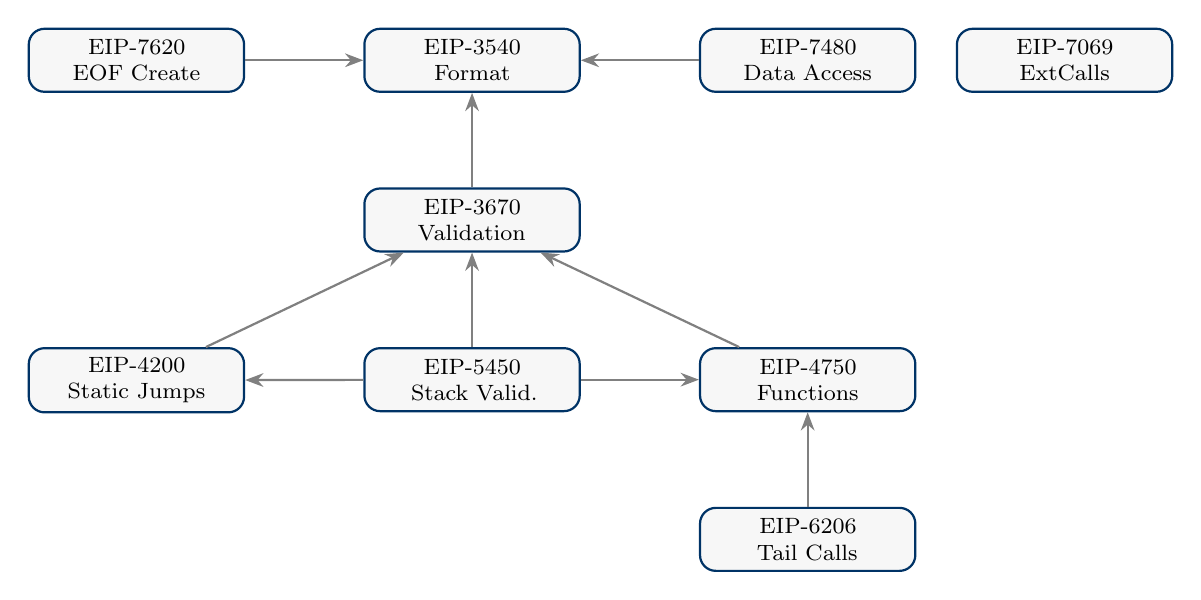
\begin{tikzpicture}[
  node distance=1.2cm and 0.5cm,
  eip/.style={rectangle, draw=primaryblue, fill=backcolour, thick, minimum size=8mm, rounded corners=2mm, text width=2.5cm, align=center, font=\footnotesize},
  arrow/.style={-Stealth, thick, gray}
]

% Core Nodes
\node[eip] (3540) {EIP-3540\\ Format};
\node[eip] (3670) [below=of 3540] {EIP-3670\\ Validation};

% Branch 1: Control Flow
\node[eip] (4200) [below left=of 3670, xshift=-1cm] {EIP-4200\\ Static Jumps};
\node[eip] (4750) [below right=of 3670, xshift=1cm] {EIP-4750\\ Functions};
\node[eip] (6206) [below=of 4750] {EIP-6206\\ Tail Calls};

% Branch 2: Stack
\node[eip] (5450) [below=of 3670] {EIP-5450\\ Stack Valid.};

% Branch 3: Features
\node[eip] (7480) [right=of 3540, xshift=1cm] {EIP-7480\\ Data Access};
\node[eip] (7069) [right=of 7480] {EIP-7069\\ ExtCalls};

% Branch 4: Creation
\node[eip] (7620) [left=of 3540, xshift=-1cm] {EIP-7620\\ EOF Create};

% Arrows
\draw[arrow] (3670) -- (3540);
\draw[arrow] (4200) -- (3670);
\draw[arrow] (4750) -- (3670);
\draw[arrow] (5450) -- (3670);
\draw[arrow] (6206) -- (4750);
\draw[arrow] (5450) -- (4200);
\draw[arrow] (5450) -- (4750);
\draw[arrow] (7480) -- (3540);
\draw[arrow] (7620) -- (3540);

\end{tikzpicture}
\caption{Dependency Graph \& Critical Path}
\end{figure}

\section{Early Prototyping Results}

To de-risk the implementation phase, we developed a functional Rust prototype (`prototype/eof`). This library serves as a reference implementation for the logic that will eventually reside in the `builtin-actors`.

\subsection{Parsing the Container}
The prototype successfully implements the recursive parsing logic required for EIP-3540. It handles the header parsing, section size validation, and the extraction of raw bytes into structured `EOFContainer` objects.

\begin{lstlisting}[language=Rust, caption=Container Parsing Logic]
pub fn parse_eof_container(bytecode: &[u8]) -> Result<EOFContainer, EOFError> {
    let mut cursor = 0;
    // Check Magic
    if bytecode.len() < 2 || bytecode[0..2] != [0xEF, 0x00] {
        return Err(EOFError::InvalidMagic);
    }
    cursor += 2;
    
    // Version Check
    if bytecode[cursor] != 0x01 {
        return Err(EOFError::InvalidVersion(bytecode[cursor]));
    }
    cursor += 1;

    // ... Section Parsing Loop ...
}
\end{lstlisting}

\subsection{Validating the Code}
We implemented the core validation pass defined in EIP-3670. This function iterates over the code section and rejects any contract containing forbidden legacy instructions.

\begin{lstlisting}[language=Rust, caption=EIP-3670 Validation Stub]
pub fn validate_eof_container(container: &EOFContainer) -> Result<(), EOFError> {
    for header in &container.header.section_headers {
        if header.kind == SectionKind::Code {
            // ... Iterate over bytes ...
            match opcode {
                INVALID | SELFDESTRUCT => return Err(EOFError::InvalidOpcode(opcode)),
                JUMP | JUMPI | PC => return Err(EOFError::JumpDestForbidden(opcode)),
                // ... 
            }
        }
    }
    Ok(())
}
\end{lstlisting}

\subsection{Simulating Static Jumps}
One of the most complex changes is the shift to relative jumps. Our prototype includes a step-function simulator that correctly calculates the target Program Counter (PC) based on the current PC and the signed 16-bit immediate value provided by the \texttt{RJUMP} instruction. This validated our understanding of the EIP-4200 arithmetic.

\section{Conclusion}

The "Pectra Phase 2" grant cycle has achieved its primary objectives. We have moved from a high-level understanding of EOFv1 to a granular, technically validated roadmap for FVM integration. 

The scoping phase confirmed that while the changes are extensive, they are well-contained within the EVM actor layer. The analysis identified key opportunities for FVM-specific optimizations, particularly regarding data loading and gas efficiency. Finally, the prototype demonstrated that the core logic—parsing, validation, and static jumps—can be implemented cleanly in Rust.

Germina Labs recommends proceeding immediately to the engineering phase, starting with the integration of the container parser into the `builtin-actors` repository. The foundation laid by this report ensures that the Filecoin network will be ready to support the next generation of secure, efficient Ethereum smart contracts.

\end{document}
